\chapter{Realization}
In order to implement the proposed solution, we have proposed a proof of concept
which is a web application built with Streamlit that demonstrates the different
features that can be offered.

The use case that we consider in this proof of concept has the following specifications:
\begin{itemize}
    \item The user can select a dataset to be added and indexed.
    \item The user can have the previously indexed datasets.
    \item The user can select a dataset, that we call a query dataset, and measure
    its similarities with the other ones.
    \item The computed similarities are presented in two sections:
    \begin{enumerate}
        \item Dataset similarity representation: It orders the dataset by their
        similarity scores with the query datasets.
        \item Column similarity representation: It shows the details of the
        column similarities between the query dataset and a dataset that the
        user selects.
    \end{enumerate}
\end{itemize}


\section{Technologies and frameworks}
In order to implement the proposed solution, we have opted for the following
technologies, tools and frameworks:
\subsection{Python}
Python is a structured, open source, multi-paradigm, multi-platform programming
language that runs on all major operating systems and computing platforms. By
offering high-level tools and an easy-to-use syntax, it greatly optimizes the
productivity of programmers and has become a leading language in exploratory
data analysis and software development.

Python has been chosen to implement this project for the following reasons:
\begin{itemize}
    \item It provides a set of libraries, in the machine learning domain, which
    simplifies the development of our project.
    \item Python manages its resources (memory, file descriptors) without the
    intervention of the programmer, by a reference counting mechanism.
    \item The Lab team of Talend has already used Python in most of their
    projects, this makes it easier to understand, collaborate, scale and
    integrate our solution in the future.
\end{itemize}

We follow up by presenting some of the used libraries during this project:

\begin{enumerate}
    \item \textbf{Numpy}:
A library used to manipulate matrices, multidimensional arrays, vectors and
polynomials, it has a large number of mathematical functions that can be applied
directly to the structures mentioned above. In this project we have used Numpy
to process matrices and arrays.
    
    \item \textbf{Jax}:
Following its definition in its official repository \citep{jax_2022}, Google JAX
is a machine learning framework for transforming numerical functions, the goal
of using this framework is to take advantage of its version of Numpy that
provides us with the possibility of doing the different calculations on GPU. It
shows up that this choice is accurate if we take in consideration the number of
matrix multiplication that we have to do in Cross-Polytope.

    \item \textbf{Pandas}:
Pandas is a python library that allows to easily manipulate data in form of data
tables that we call DataFrame with column and row labels. It provides us with
some interesting easily used features to read, analyze and complete some
preprocessing operations.

    \item \textbf{IGraph}:
It is a library allowing to define and manipulate graphs, it is written in C
programming language and can be used with Python or R. We use it in our solution
to define the graphs representing the results of similarities between columns
and between datasets

    \item \textbf{Plotly}:
Plotly is a complete library for creating static, animated and interactive
visualizations in Python. It is used in our solution to represent the graphs
defined with IGraph with interactive figures in the Streamlit application.

    \item \textbf{Transformers}:
We use the Transformers library which is a state of the art pre-trained model
library for natural language processing (NLP). The library currently contains
pre-trained model weights, user scripts and conversion utilities: Bert,
Roberta\ldots.

\end{enumerate}


\subsection{Streamlit}
It is an open source framework in Python language dedicated for data scientists
and machine learning engineers to create complete web applications in a short
time as it provides a set of components that we need to have an interactive
layout. It also provides a compatibility with different Python libraries which
make it easier for building demonstrations that are not exclusive to data
scientists.

Streamlit has also a cloud platform that gives its users the possibility to
deploy, manage and share their apps.

\subsection{TensorFlow Hub}
It is a repository of trained machine learning models ready for downloading,
fine-tuning or reusing in different projects, with the possibility to be deployed
everywhere.

We used this library to test different embedding models and choose the most
suitable one in order to get a representation for the textual columns.


\section{Architecture}
The proof of concept has been implemented using two layers, the logic layer
which is responsible for providing the features of indexation, storing, querying
and similarity representation, while the second layer, the presentation layer,
is responsible of building the user interface that offers the user the
possibility to add and index a new dataset, display the stored indexes, look up
for similarities and get their representations.

The figure \ref{fig:folder_organization} shows the organization of the project
folder where $data\_fingerprinting$ represents the logic layer, and
$visual\_demo$ represents the presentation layer.

\begin{figure}[h]
    \begin{subfigure}{.4\textwidth}
        \centering
        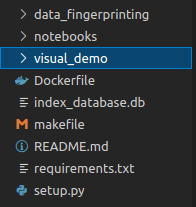
\includegraphics{realization/application.png}
    \end{subfigure}
    \begin{subfigure}{.4\textwidth}
        \centering
        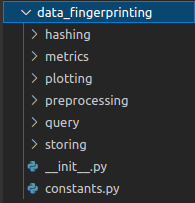
\includegraphics{realization/logic.png}
    \end{subfigure}
    \begin{subfigure}{.4\textwidth}
        \centering
        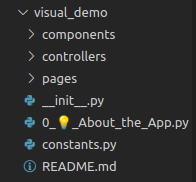
\includegraphics{realization/presentation.png}
    \end{subfigure}
    \caption{The organization of the project folders.}
    \label{fig:folder_organization}
\end{figure}

The logic layer contains the five components introduced in the class diagram
in section \ref{sect:concep_implementation} which are: Preprocessing, Hashing,
Query, Plotting, and Storing. We use SQLite database for storing and reading the
indexes, it mainly interacts with the Storing component. The presentation layer
is divided into two components, the view component to build the user interface
which is a multi-page layout, and the controller component which provides all
the interactions between the view component and the logic layer.

The figure \ref{fig:architecture} shows the architecture of the proof of concept
built to demonstrate the functioning of the similarity detection process with
LSH.

\begin{figure}[h]
    \centering
    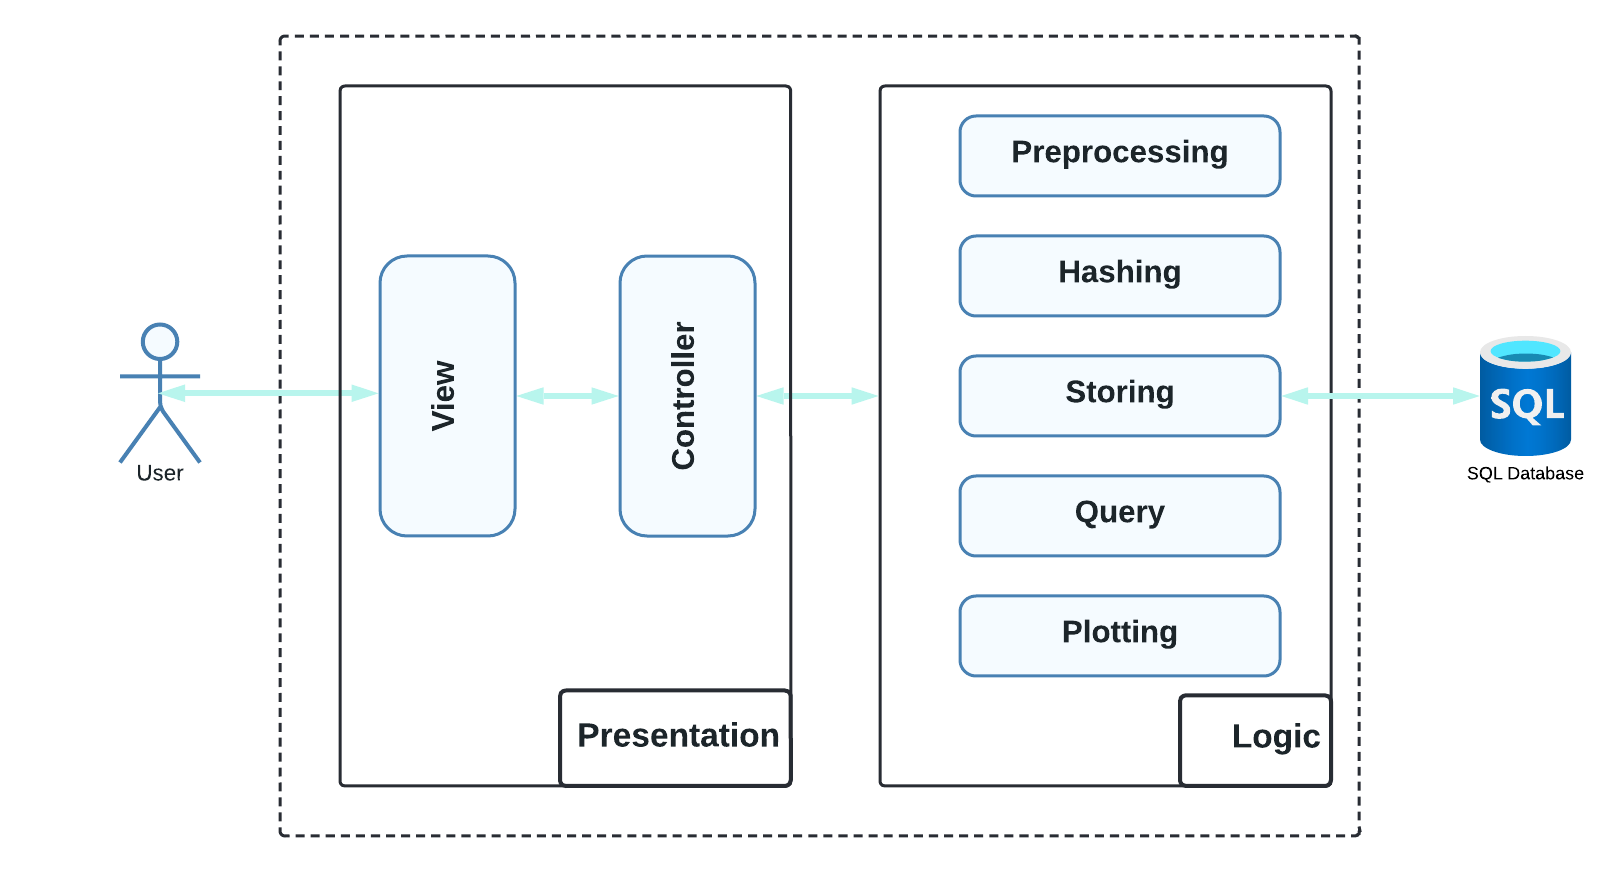
\includegraphics[width=\textwidth]{realization/architecture.png}
    \caption{The architecture of the proof of concept}
    \label{fig:architecture}
\end{figure}